% Proxies stand in for multiple versions, intercept all access, and forward to the correct version.


\chapter{Implementation} \label{chapter:IMPLEMENTATION}

This chapter describes how we used the ECMAScript 6 proxies\footnote{\url{http://wiki.ecmascript.org/doku.php?id=harmony:direct_proxies}, accessed February 3rd, 2014} to implement version-aware references for the Lively Kernel.
It presents the proxy's behavior and shows how proxies are inserted for ordinary references using source transformations.
The chapter also presents implemented workarounds for the current state of ECMAScript 6 proxies.
It concludes with current limitations.

\section{ECMAScript 6 Proxies as Version-aware References} \label{sec:IMPLEMENTATION:1}

This section first describes the proxies proposed with the next version of JavaScript's standard.
It then explains how the proxies are used in our implementation.

\subsection{ECMAScript 6 Proxies by Example} \label{subsec:IMPLEMENTATION:1.1}

The ECMAScript 6 proxies stand in for objects and intercept all kinds of object interactions.

The object a proxy stands in for is its \emph{target}.
The behavior of a proxy is controlled by a separate \emph{handler} object.
Target and handler are required when a proxy is created as in the following example:
\iffalse
\begin{verbatim}\fi
\begin{code}{}{}
var proxy = new Proxy(target, handler);
\end{code}
\iffalse
\end{verbatim}\fi

The handler can implement \emph{traps}, which are specific methods.
Traps are called when a proxy intercepts corresponding object interactions.
For example, the \emph{get} trap is called for property reads.
With these traps, the handler specifies how the proxy reacts on object interaction.

\iffalse
\begin{verbatim}\fi
\begin{code}[lst:loggingProxy]{Using a proxy to log property reads to an object.}{float,numbers=left}
var client = {},
    server = {openSecret: "I don't like Mondays"},
    handler = {
        get: function(target, name) {
            console.log(name + ' was read at ' + Date());
            
            return target[name];
        }
    }

client.server = new Proxy(server, handler);
\end{code}
\iffalse
\end{verbatim}\fi

Listing~\ref{lst:loggingProxy} shows an example, in which a proxy is used to log property reads.
A \lstinline{client} object is connected to a \lstinline{server} object via a proxy, as shown in Figure~\ref{fig:LoggingProxy}:
The \lstinline{client}'s \lstinline{server} property is a reference to a proxy and that proxy's target is the \lstinline{server}.

\begin{figure}[h]
    \centering
    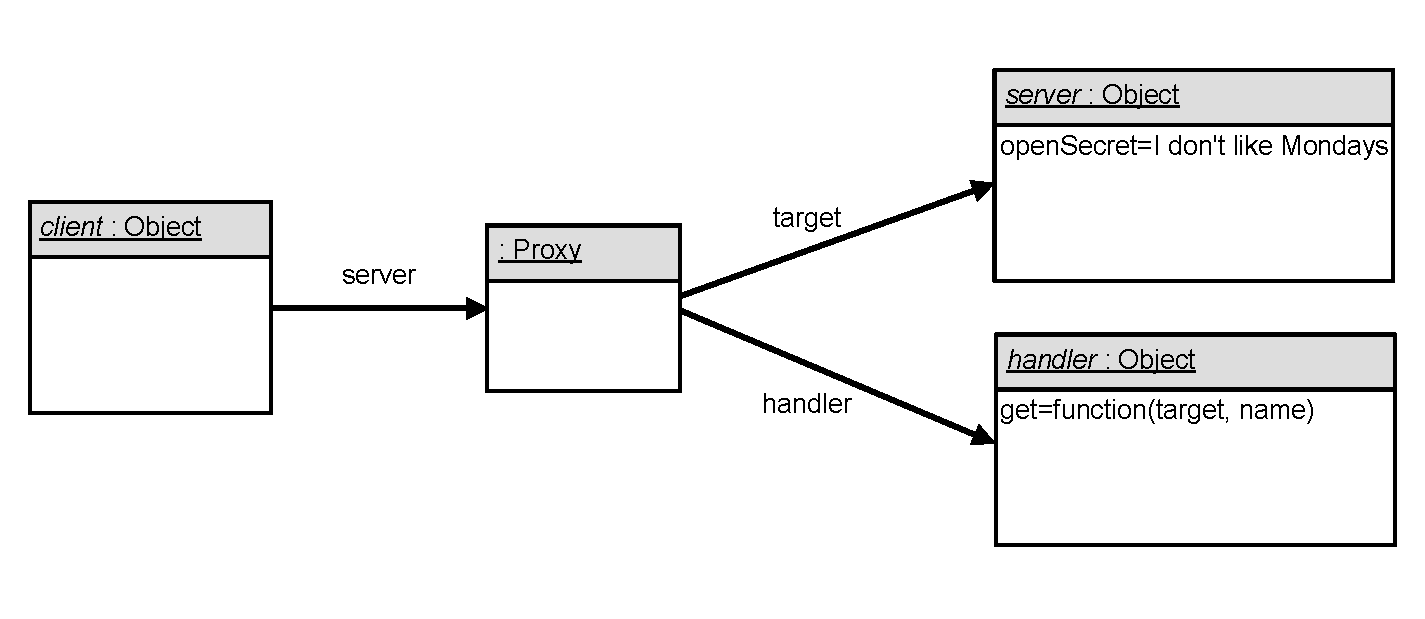
\includegraphics[width=\textwidth]{figures/5_implementation/1_loggingProxy.pdf}
    \caption{A \lstinline{client} object has access to a \lstinline{server} object via a proxy.}
    \label{fig:LoggingProxy}
\end{figure}

The proxy's \lstinline{handler} object implements a \lstinline{get} trap.
The \lstinline{get} trap receives two arguments when called: \lstinline{target} and \lstinline{name}.
The \lstinline{target} parameter refers to the proxy's target object.
The \lstinline{name} parameter refers to the name of the property that was read.
In Listing~\ref{lst:loggingProxy}, the \lstinline{get} trap logs the property read (Line~5), then forwards the read to the \lstinline{target} object and returns the result (Line~7).
Therefore, reading a property of the server object via the proxy as shown in Listing~\ref{lst:propertyRead} would print a log statement similar to the following: ``openSecret was read at Sat May 10 2014 23:00:54 GMT+0200 (CEST)''.

\iffalse
\begin{verbatim}\fi
\begin{code}[lst:propertyRead]{Reading the \lstinline{openSecret} property of a \lstinline{client} object's \lstinline{server} property.}{float}
client.server.openSecret;
\end{code}
\iffalse
\end{verbatim}\fi

A handler object can implement traps for many different kinds of object interactions.
Table~\ref{table:traps} lists all possible traps with their parameters.

\begin{table}[h]
\begin{center}
\begin{tabular}{|l|l|r|}
\hline
get: function(target, name, receiver) \\ \hline
set: function(target, name, value, receiver) \\ \hline
apply: function(target, thisArg, args) \\ \hline
construct: function(target, args) \\ \hline
has: function(target, name) \\ \hline
hasOwn: function(target, name) \\ \hline
defineProperty: function(target, name, desc) \\ \hline
deleteProperty: function(target, name) \\ \hline
getOwnPropertyDescriptor: function(target,name) \\ \hline
getOwnPropertyNames: function(target) \\ \hline
getPrototypeOf: function(target) \\ \hline
freeze: function(target) \\ \hline
seal: function(target) \\ \hline
preventExtensions: function(target) \\ \hline
isFrozen: function(target) \\ \hline
isSealed: function(target) \\ \hline
isExtensible: function(target) \\ \hline
enumerate: function(target) \\ \hline
keys: function(target) \\ \hline
\end{tabular}
\caption[Table caption text]{Traps that proxy handlers can provide.}
\label{table:traps}
\end{center}
\end{table}

The traps fire either when a proxy is accessed with JavaScript operators or when it is passed to meta-programming facilities.
For example, the \lstinline{apply} trap fires when a proxied function is applied as in the following example:
\iffalse
\begin{verbatim}\fi
\begin{code}{}{}
proxy();
\end{code}
\iffalse
\end{verbatim}\fi
The \lstinline{preventExtensions} trap fires when a proxy is passed to the \lstinline{preventExtensions} function of the global \lstinline{Object}, which prevents subsequentely adding new properties to an object.
The trap would be triggered by statements such as the following:
\iffalse
\begin{verbatim}\fi
\begin{code}{}{}
Object.preventExtension(proxy);
\end{code}
\iffalse
\end{verbatim}\fi

When no trap is provided for a kind of object interactions, the proxy forwards the interaction transparently to the target.

The \lstinline{apply} trap and the \lstinline{construct} traps are only called, when a proxy's target is a function.

\paragraph{Using the Proxies as Virtual Objects}
The proxies require target objects to which they forward by default.
However, when a proxy's handler implements all traps, all intercepted interactions can be handled by the traps without forwarding to the target object.
Therefore, even though proxies have target objects, the target objects do not have to be accessed with any object interactions.
\\
This solution for using the proxies as virtual objects is also proposed by the official documentation\footnote{\url{http://wiki.ecmascript.org/doku.php?id=harmony:direct\_proxies\#virtual_objects}, accessed May 11, 2014}.



\subsection{Using the Proxies for Object Versioning} \label{subsec:IMPLEMENTATION:1.2}

The proxies stand in for multiple versions of an object in our implementation.
They forward all object interactions to a dynamically chosen version.

Figure~\ref{fig:VersioningProxy} exemplifies our usage of the proxies.
In the example, a proxy stands in for two versions of an \lstinline{address} object: The proxy's handler holds a reference to a \lstinline{versions} object, which in turn refers to the versions of the \lstinline{address} object.
The proxy's target is ommited from Figure~\ref{fig:VersioningProxy} as we used the proxies as virtual objects.
Therefore, they do not forward to their targets.

\begin{figure}[h]
    \centering
    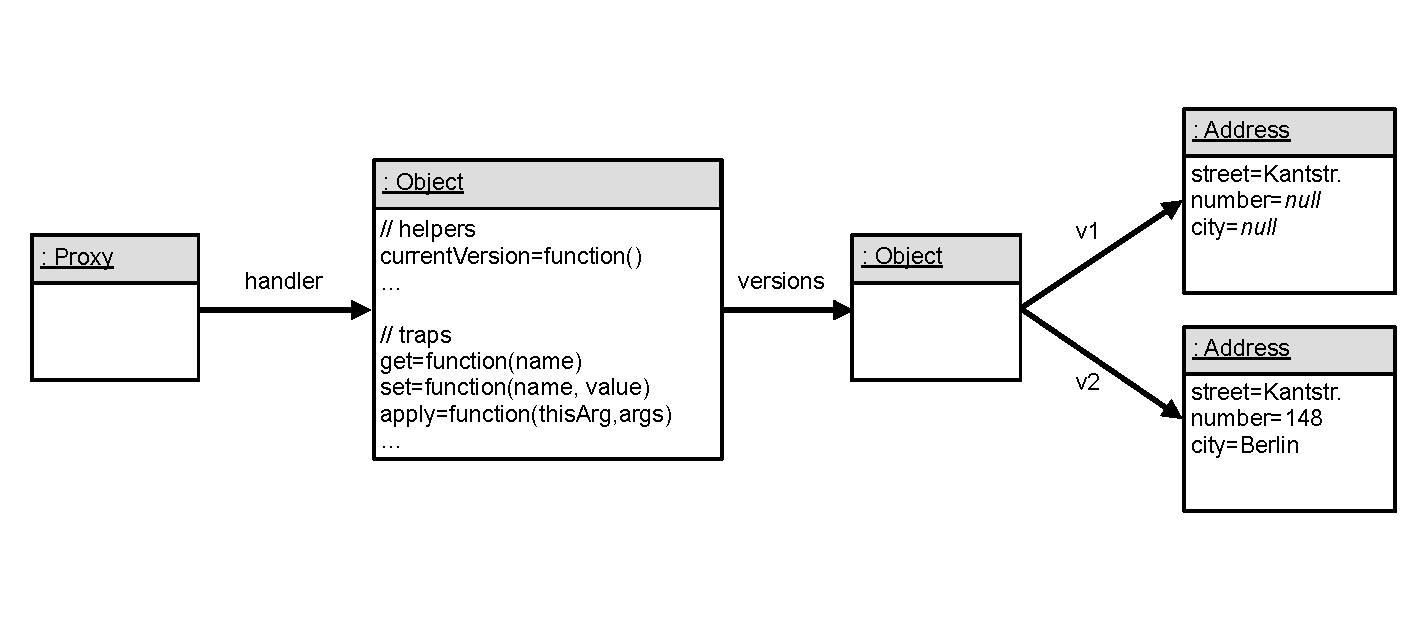
\includegraphics[width=\textwidth]{figures/5_implementation/2_versioningProxy.pdf}
    \caption{A proxy with a handler that forwards to two versions of an \lstinline{address} object.}
    \label{fig:VersioningProxy}
\end{figure}

Our handler uses all traps to forward to the current version of an object.
For example, its \lstinline{get} trap works as shown in Listing~\ref{lst:getTrap}.

\iffalse
\begin{verbatim}\fi
\begin{code}[lst:getTrap]{The handler's \lstinline{get} trap.}{float,numbers=left}
get: function(dummyTarget, name) {
    var version = this.currentVersion();
    
    return version[name];
}
\end{code}
\iffalse
\end{verbatim}\fi

First, the trap retrieves the current version of the object using a helper function, which is named \lstinline{currentVersion} (Line~2).
Subsequentely, the trap reads the property from the current version and returns the result (Line~4).

The \lstinline{currentVersion} function chooses one of the versions of the object the proxy stands in for.
It does so according to the version of the system.
The version of the system is available globally as \lstinline{lively.CurrentVersion}.
It is an ordinary JavaScript object with three properties: an \lstinline{ID}, a \lstinline{predecessor}, and a \lstinline{successor}.
The \lstinline{currentVersion} function uses the \lstinline{ID} property to look up the correct version in its \lstinline{versions} object.

Object versions of previous system versions are not allowed to change.
However, when a version of an object is not changed in versions of the system, an object version of a previous system version reflects the current state.
Therefore, objects are not copied when they are not changed.
Instead, the \lstinline{currentVersion} function retrieves the latest available version as shown in Listing~\ref{lst:currentVersion}.

\iffalse
\begin{verbatim}\fi
\begin{code}[lst:currentVersion]{The handler's \lstinline{currentVersion} method.}{float,numbers=left}
currentVersion: function() {
    var objectVersion,
        systemVersion = lively.CurrentVersion;
    
    while(!objectVersion && systemVersion) {
        objectVersion = this.versions[systemVersion.ID];

        systemVersion = systemVersion.previousVersion;
    }
    
    return objectVersion;
}
\end{code}
\iffalse
\end{verbatim}\fi

Traps that intercept changes are not allowed to forward to object versions of previous system versions.
Instead, they need to make sure that a version of the object exists for the current system version.
If such a version does not exist, the latest available version is copied and stored in the \lstinline{versions} object.

Listing~\ref{lst:versionForWriteAccess} shows the \lstinline{versionForWriteAccess} function that always returns an object version for the current system version.
The function is used by all traps that intercept changes, which are listed in Table~\ref{table:writeTraps}.
The \lstinline{apply} trap is included in this list, because built-in array functions such as \lstinline{push} and \lstinline{pop} are mutating.

\iffalse
\begin{verbatim}\fi
\begin{code}[lst:versionForWriteAccess]{The handler's \lstinline{versionForWriteAccess} method.}{float,numbers=left}
versionForWriteAccess: function() {
    var newVersion;
    
    if (!this.versions[lively.CurrentVersion.ID]) {
        newVersion = this.copyObject(this.currentVersion());
        
        this.versions[lively.CurrentVersion.ID] = newVersion;
    }
    
    return this.currentVersion();
},
\end{code}
\iffalse
\end{verbatim}\fi

\begin{table}[h]
\begin{center}
\begin{tabular}{|l|l|r|}
\hline
set: function(target, name, value, receiver) \\ \hline
defineProperty: function(target, name, desc) \\ \hline
deleteProperty: function(target, name) \\ \hline
freeze: function(target) \\ \hline
seal: function(target) \\ \hline
preventExtensions: function(target) \\ \hline
apply: function(target, thisArg, args) \\ \hline
\end{tabular}
\caption[Table caption text]{Traps that intercept changes.}
\label{table:writeTraps}
\end{center}
\end{table}

The remaining traps select the version to forward to using the \lstinline{currentVersion} function.

Given the \lstinline{currentVersion} and the \lstinline{versionForWriteAccess} functions, the current version of the system is written as long as it is referred to by \lstinline{lively.CurrentVersion}.
To re-establish a different version, only this reference has to be changed.
Changing the global version is an undo, redo, or commit depending on whether the version is set to a previous, following, or new version.
For this, the system provides the functions \lstinline{lively.undo} (Listing~\ref{lst:undo}), \lstinline{lively.redo} (Listing~\ref{lst:redo}), and \lstinline{lively.commit} (Listing~\ref{lst:commit}).

\iffalse
\begin{verbatim}\fi
\begin{code}[lst:undo]{The \lstinline{lively.undo} method.}{float,numbers=left}
undo: function() {
    var predecessor = lively.CurrentVersion.predecessor;
    
    if (!predecessor) {
        throw new Error('Can\'t undo: No previous version.');
    }
    
    lively.CurrentVersion = predecessor;
}
\end{code}
\iffalse
\end{verbatim}\fi

\iffalse
\begin{verbatim}\fi
\begin{code}[lst:redo]{The \lstinline{lively.redo} method.}{float,numbers=left}
redo: function() {
    var successor = Lively.CurrentVersion.successor;
    
    if (!successor) {
        throw new Error('Can\'t redo: No next version.');
    }
    
    lively.CurrentVersion = successor;
}
\end{code}
\iffalse
\end{verbatim}\fi

\iffalse
\begin{verbatim}\fi
\begin{code}[lst:commit]{The \lstinline{lively.commit} method.}{float,numbers=left}
commit: function() {
    var predecessor = lively.CurrentVersion,
        newVersion;
    
    newVersion = {
        ID: predecessor.ID + 1,
        predecessor: predecessor,
        successor: null
    };
    predecessor.successor = newVersion;
    
    lively.CurrentVersion = newVersion;
}
\end{code}
\iffalse
\end{verbatim}\fi

Using a global version of the system is reasonable as JavaScript is executed single-threaded and scheduled cooperatively by the JavaScript engines.
While a script runs, the global version cannot be changed by another script.

 
\subsubsection{Scope of the Versioning} \label{subsubsec:IMPLEMENTATION:5.2.1}

Using the proxies allows for versioning JavaScript objects.
However, certain host objects cannot be versioned with our implementation.
These include the objects that represent the elements of the browser's \ac{dom}.
Some of \ac{dom} objects cannot be copied.
For this reason, it is not possible to create multiple versions of them.
Moreover, the \ac{dom} objects are referred to from the browser's \ac{dom}, which is external to the JavaScript runtime and which, thus, does not use version-aware references.
However, this is not a problem, because the state of the \ac{dom} can be derived from the Lively Kernel's morph objects.
Therefore, we update the \ac{dom} from the current set of visible morphs when the system version changes.
Besides these host objects, all objects that are accessed through our proxies are versioned with the system versions.





\section{Proxies For All Mutable JavaScript Objects}

To be able to re-establish the entire state with our versioning, our proxies need to be used to access all objects, arrays, and functions.
This is necessary because objects, arrays, and functions are mutable in JavaScript.
In fact, functions and arrays are objects.
They can have arbitrary properties.

Our implementation changes the return values of all expressions that create new objects.
Instead of letting these expressions return references to the new objects, the expressions return references to proxies for the objects.
As a result, references to proxies are passed around instead of references to objects so that all access goes through the proxies.

In JavaScript, there are three categories of expressions that create new objects: 
\begin{itemize}
    \item literal expressions: e.g. \lstinline|{age: 12}|
    \item constructor functions: e.g. \lstinline|new Person(12)|
    \item specific built-in functions: e.g. \lstinline|Object.create(prototype, {age: 12})|
\end{itemize}

Our implementation uses source transformations and proxy traps to have these expression return proxies.


\subsection{Transforming Literal Expressions}

We use source transformations to wrap literal expressions into calls to a \lstinline{proxyFor} function.
The \lstinline{proxyFor} function returns a proxy for its argument.
The transformations for literal objects, arrays, and functions are shown in Table~\ref{table:literalTransforms}.

\begin{table}[h]
\begin{center}
\begin{tabular}{| l | l | l |}
\hline
Type & Input & Output \\ \hline
\emph{Objects} & \lstinline|{name: 'James', age: 24}| & \lstinline|proxyFor(name: 'James', age: 24)| \\ \hline
\emph{Arrays} & \lstinline|[person1, person2]| & \lstinline|proxyFor([person1, person2])| \\ \hline
\emph{Functions} & \lstinline|function (a, b) {..}| & \lstinline|proxyFor(function (a, b) {..})| \\ \hline
\end{tabular}
\end{center}
\caption[Table caption text]{Transforming literal objects, arrays, and functions.}
\label{table:literalTransforms}
\end{table}

However, some literal forms cannot be wrapped into function calls without introducing problems.
In particular, function declarations and accessor functions need to be handled differently.


\subsubsection{Function Declarations}

A \emph{function declaration} is a function literal that creates a named function and makes it available by the name.
It does not need to be assigned to a variable to be available in the surrounding scope.
The following statement is a function declaration:
\iffalse
\begin{verbatim}\fi
\begin{code}{}{}
function add(a, b) {return a + b}
\end{code}
\iffalse
\end{verbatim}\fi

In contrast, a \emph{function expression} creates a function that needs to be assigned to a variable to be accessible.
The following statement assigns a function expression to a variable:
\iffalse
\begin{verbatim}\fi
\begin{code}{}{}
var subtract = function(a, b) {return a - b}
\end{code}
\iffalse
\end{verbatim}\fi

Function expressions can create anonymous and named functions.
The example above creates an anonymous function.
The following example assigns a named function to a variable:
\iffalse
\begin{verbatim}\fi
\begin{code}{}{}
var multiply = function multiply(a, b) {return a * b}
\end{code}
\iffalse
\end{verbatim}\fi

An anonymous function is always a function expression.
A named function is either a function expression or a function declaration, depending on where it is expressed.
A function declaration cannot be nested into other statements such as variable assignments.
It has to start with the \lstinline{function} keyword.

Therefore, when a function declaration is wrapped into a function call, it becomes a function expression.
The function would no longer be available by its name in the surrounding scope.
For this reason, the function declarations that are wrapped into calls to the \lstinline{proxyFor} function are assigned to matching variable names.
Table~\ref{table:funcTransform} shows an example for this transformation.

\begin{table}[h]
\begin{center}
\begin{tabular}{| l | l | l |}
\hline
Input & Output \\ \hline
\lstinline|function div() {}| & \lstinline|var div = proxyFor(function div() {})| \\ \hline
\end{tabular}
\end{center}
\caption[Table caption text]{Transforming a function declaration.}
\label{table:funcTransform}
\end{table}

In addition, because function declarations get hoisted in JavaScript, transformed function declarations are moved to the beginning of the defining scope.


\subsubsection{Accessor Functions}

Accessor functions are functions that are executed transparently instead of property reads or writes.
Listing~\ref{lst:accessorOriginal} shows an example in which an accessor function is used to allow reading a \lstinline{person}'s \lstinline{age} even though the \lstinline{person} object only has a \lstinline{birthdate} property.

\iffalse
\begin{verbatim}\fi
\begin{code}[lst:accessorOriginal]{An object literal with accessor function.}{float,numbers=left}
var person = {
    birthdate: new Date(1984,27,5),
    get age() {
        return ageToday(this.birthdate);
    }
}
\end{code}
\iffalse
\end{verbatim}\fi

Wrapping the accessor function into the \lstinline{proxyFor} function would not yield valid JavaScript syntax.
However, accessor functions can also be defined with the \lstinline{Object.defineProperty} function.
Therefore, the object is created without accessor functions and the accessor function defined separately using \lstinline{Object.defineProperty}.
Both the object and the accessor functions can be wrapped into calls to the \lstinline{proxyFor} function when expressed in this way.
Listing~\ref{lst:accessorTransformed} shows the result of transforming the example in Listing~\ref{lst:accessorOriginal}.
The new object is created in an anonymous functions that is applied directly.
In this anonymous function, the new object is assigned to a variable called \lstinline{newObject}.
This allows to have the object be available in a variable for the subsequent \lstinline{Object.defineProperty}-function call without polluting the variable bindings of the originally surrounding scope.

\iffalse
\begin{verbatim}\fi
\begin{code}[lst:accessorTransformed]{The result of transforming an object literal with accessor function.}{float,numbers=left}
var person = function() {
    var newObject = lively.proxyFor({
        birthdate: new Date(1984,27,5);
    });
    Object.defineProperty(newObject, "age", {
        get: lively.proxyFor(function age() {
            return ageToday(this.birthdate);
        })
        enumerable: true,
        configurable: true
    });
    return newObject;
}();
\end{code}
\iffalse
\end{verbatim}\fi



\subsection{Returning Proxies from Constructor Functions} 

When functions are used as constructors, they need to return proxies.
In JavaScript, all functions can be used as constructors and create objects when called with the \lstinline{new} operator.
Listing~\ref{lst:constructorFunction} shows how a literal function is used to construct a new object.

\iffalse
\begin{verbatim}\fi
\begin{code}[lst:constructorFunction]{Applying a function with the \lstinline{new} operator.}{float, numbers=left}
function Person() {}
var someone = new Person();
\end{code}
\iffalse
\end{verbatim}\fi

We use the \lstinline{construct} trap to return proxies from proxied functions used as constructors.
Listing~\ref{lst:constructTrap} shows the \lstinline{construct} trap of our proxy handlers.

\iffalse
\begin{verbatim}\fi
\begin{code}[lst:constructTrap]{The handler's \lstinline{contruct} trap.}{float,numbers=left}
construct: function(dummyTarget, args) {
    var constructor, prototype, newObject, result;
    
    constructor = this.currentVersion()
    
    prototype = constructor.prototype ? constructor.prototype : {}    
    newObject = Object.create(prototype);
    
    result = constructor.apply(newObject, args);
    
    return proxyFor(result ? result : newObject);
}
\end{code}
\iffalse
\end{verbatim}\fi

The \lstinline{construct} trap does the following:
\begin{enumerate}
    \item It retrieves the current version of the constructor (Line~4).
    \item It creates a new object with the correct prototype (Line~7).
    \item It applies the constructor to the new object (Line~9).
    \item It returns a proxy for either the return value of the constructor function or, in case the constructor did not return a value, the new object (Line~11).
\end{enumerate}

This way, all proxied functions return proxies when used as constructors.
With the transformations of literal expressions presented in the previous subsection all literal functions are accessed through proxies.\\
However, there are also functions built into the JavaScript engines.
These are not created from function literals and, therefore, cannot be proxied by transforming literals.


\subsection{Wrapping Built-in Functions}

Some built-in functions can be used to create new objects.
For example, the built-in constructors \lstinline{Object} and \lstinline{Array} can be used to create new objects and arrays.
They return new objects when called with the \lstinline{new} operator and when called without.\\
Other global functions that allow creating new objects include, for example, \lstinline{Object.create} and \lstinline{eval}.
The \lstinline{Object.create} function takes an object as argument, uses the argument as prototype of a new object, and returns the new object.
The \lstinline{eval} function takes a string as argument it.
It evaluates the string as JavaScript code and, depending on the code string, can return new objects and even object graphs.


\subsubsection{Wrapping Built-in Constructor Functions}

We transform the built-in constructor functions by wrapping each into calls to the \lstinline{proxyFor} function.
Table~\ref{table:transformingBuiltInConstructors} shows this with two examples for the global \lstinline{Object} function.

\begin{table}[h]
\begin{center}
\begin{tabular}{| l | l | l |}
\hline
Input & Output \\ \hline
\lstinline|Object()| & \lstinline|proxyFor(Object)()| \\ \hline
\lstinline|new Object()| & \lstinline|new proxyFor(Object)()| \\ \hline
\end{tabular}
\end{center}
\caption[Table caption text]{Transforming built-in constructors.}
\label{table:transformingBuiltInConstructors}
\end{table}

The global symbols that are wrapped into calls to the \lstinline{proxyFor} are: \lstinline{Array}, \lstinline{Boolean}, \lstinline{Date}, \lstinline{Function}, \lstinline{Iterator}, \lstinline{Number}, \lstinline{Object}, \lstinline{RegExp}, \lstinline{String}, \lstinline{JSON}, \lstinline{Math}, \lstinline{Intl}, \lstinline{window}, \lstinline{document}, \lstinline{XMLHttpRequest}, \lstinline{Worker}, \lstinline{XMLSerializer}.

Therefore, when these function objects are used as constructors, the \lstinline{construct} trap is called and returns proxies for the new objects as explained in the previous subsection.
As these functions also create objects when called without the \lstinline{new} operator, we also have the \lstinline{apply} trap return proxies.
Therefore, the last line of the \lstinline{apply} trap is:
\iffalse
\begin{verbatim}\fi
\begin{code}{}{}
this.ensureProxied(result);
\end{code}
\iffalse
\end{verbatim}\fi

When the argument to \lstinline{ensureProxied} is already a proxy or an immutable value such as a string or a number, it returns the argument unchanged.
When the argument is however an object, an array, or a function, the \lstinline{ensureProxied} returns a proxy for that object.
This distinction is necessary as the \lstinline{apply} trap is all functions, not only built-in constructors.


\paragraph{Proxy Table}
With our solution each occurrence of a built-in constructor is wrapped into a separate call to the \lstinline{proxyFor} function.
Therefore, the same function objects are passed to the \lstinline{proxyFor} function multiple times.
To nevertheless return the same proxies for the same objects, a map is used to associate objects with their proxies.
This \emph{Proxy Table} is a weak-key map.
It does not prevent garbage collection of objects used as keys when the proxies to the objects get garbage collected.\\
Using the same proxies for the same objects is not only an optimization, but necessary for identity checks.
As a result of using the Proxy Table, the following statement returns \lstinline{true} for an arbitrary \lstinline{obj} object:
\iffalse
\begin{verbatim}\fi
\begin{code}{}{}
proxyFor(obj) === proxyFor(obj);
\end{code}
\iffalse
\end{verbatim}\fi



\subsubsection{Wrapping Other Built-In Functions}

Besides the built-in constructors, other built-in functions that return new objects need to return proxies as well.
For example, the following statement needs to return a proxy:
\iffalse
\begin{verbatim}\fi
\begin{code}{}{}
Object.create(proto)
\end{code}
\iffalse
\end{verbatim}\fi

In addition to the \lstinline{construct} trap and the \lstinline{apply} trap, we also have the \lstinline{get} trap return proxies.
Analogous to the \lstinline{apply} trap, the last line of the \lstinline{get} trap is:
\iffalse
\begin{verbatim}\fi
\begin{code}{}{}
this.ensureProxied(result);
\end{code}
\iffalse
\end{verbatim}\fi


Therefore, proxies for objects always return proxies for the object's properties.
As a result, when the built-in constructor \lstinline{Object} gets wrapped into a call to the \lstinline{proxyFor} function as with the transformations presented above, reading its \lstinline{create} property returns a proxy for the property.
Furthermore, this proxy's \lstinline{construct} trap also returns a proxy when applied.
Thus, the following statement returns a proxy for the newly created object:
\iffalse
\begin{verbatim}\fi
\begin{code}{}{}
proxyFor(Object).create(proto);
\end{code}
\iffalse
\end{verbatim}\fi

Therefore, the previous transformations are sufficient to have all functions of the globals return proxies.

The \lstinline{eval} function, however, is handled differently.
It can return object graphs for the string argument provided.
For example, the following statement returns an object with a \lstinline{address} property, which is in turn an object:
\iffalse
\begin{verbatim}\fi
\begin{code}{}{}
eval("{age: 12, address: {street: 'Kantstr', city: 'Berlin'}}")
\end{code}
\iffalse
\end{verbatim}\fi

It is not sufficient to proxy object the \lstinline{eval} function returns.
Instead, the object also needs to access its \lstinline{address} property via a proxy.\\
Moreover, the code passed to \lstinline{eval} could access built-in constructors or itself use the \lstinline{eval} function.
For this reason, we pass the string argument of the \lstinline{eval} function through our source transformations first.

The built-in functions could be overwritten globally to return proxies for the new objects, but our implementation of object versioning is itself just a JavaScript library and makes use of the built-in types.
Additionally, at the time of writing, some JavaScript engines do not allow to overwrite particular built-in functions and we want our implementation of object versioning to work in every JavaScript engine that supports the ECMAScript 6 Direct Proxies.

\subsubsection{Implementation of Source Transformations}

Our implementation uses \emph{UglifyJS}\footnote{\url{http://github.com/mishoo/UglifyJS2}, accessed March 12, 2014} for all source transformations.
UglifyJS parses source code without relying on JavaScript exceptions.
Therefore, when code is transformed before evaluation and the transformation steps do not yield exceptions that could be caught by an open debugger.
In addition, UglifyJS supports Source Maps\footnote{\url{https://docs.google.com/document/d/1U1RGAehQwRypUTovF1KRlpiOFze0b-_2gc6fAH0KY0k/edit\#heading=h.ue4jskhddao6}, accessed May 2, 2014}.
This allows the browser's developer tools to present the original sources, even though transformed code is executed.





\section{Workarounds for the Current State of the ECMAScript 6 Proxies} \label{sec:IMPLEMENTATION:4}

Certain workarounds are required due to the preliminary implementation of ECMAScript 6 proxies in the JavaScript engines.

\paragraph{ECMAScript 6 Specification}
ECMAScript 6 will be the next version of JavaScript.
Its specification has not yet been finalized.
Drafts of it are released periodically with a target release date of December 2014\footnote{http://github.com/rwaldron/tc39-notes/blob/48c5d285bf8bf0c4e6e8bb0c02a7c840c01cd2ff/es6/2013-03/mar-13.md\#416-current-status-of-es6, accessed May 12, 2014}.
The current draft is Revision 24~\cite{Ecma2014ES6}.
It includes the proposal of the proxies we used for our implementation.

\paragraph{ECMAScript 6 Implementation}
The JavaScript engines used by Chrome and Firefox provide preliminary implementations for some of the ECMAScript 6 features.
They implement two different deprecated proposals of the proxy \ac{api}.
However, the \emph{harmony-reflect} library\footnote{\url{http://github.com/tvcutsem/harmony-reflect}, accessed February 3, 2014, used version 0.0.11} provides the current \ac{api} on top of the implemented states.
Our implementation uses the \emph{harmony-reflect} library and, thereby, works in Chrome and Firefox.

However, even with the library, three issues need to be addressed with technical workarounds:

\begin{enumerate}
    \item The proxies have to be provided with an actual target, even when implementing virtual objects, and consistency invariants compare return values of the traps to the state of the actual target. 
    \item The proxies do not intercept the \lstinline{instanceof} operator, but always delegate to the current target.
    \item Certain built-in JavaScript functions dont handle proxies correctly.
\end{enumerate}

These workarounds might no longer be necessary once the ECMAScript 6 standard gets finalized and fully implemented by the JavaScript engines. 


\subsection{Disabling Target Object Invariants}

\subsubsection{Problem}
As explained in Section~\label{subsec:IMPLEMENTATION:1.1}, the proxies as available in Chrome require a fixed target object, even though the current ECMAScript 6 draft says otherwise\footnote{\url{http://people.mozilla.org/~jorendorff/es6-draft.html\#sec-proxy-object-internal-methods-and-internal-slots}, accessed April 15, 2014}.
Therefore, even in case the proxies are used as \emph{virtual objects}, they still forward to a particular object by default.
Moreover, the proxies are designed to ensure invariants between the return values of traps and the target's state~\cite{Cutsem2013TRP}.
For example, when an object's properties are made immutable through the \lstinline{Object.freeze} function, invariants ensure that the target object has in fact been frozen, even if the trap delegates the operation to another object such as one of our versions of an object.
Another invariant ensures that immutable values of the target object are reported by the traps.
Therefore, the \emph{get}-trap has to report the values of the target object when it previously has been frozen.
That is, in our case, configuring any property as immutable would effectively make that property immutable for all versions.
Moreover, reading the property in a version where the property is different from the immutable target's property would raises inconsistency errors.

\subsubsection{Solution}
For this reason, we adapted our copy of the \emph{harmony-reflect} library.
In particular, the \lstinline{Proxy} constructor function takes a third argument.
This argument is a boolean that indicates whether a proxy is standing in for one target object or is a virtual object.
This boolean flag is then used to disable all consistency checks when a proxy is used as virtual object.


\subsubsection{Discussion}

The proxy constructor still requires an actual object as \emph{target} object.
This target object is used for object interactions that are not intercepted by any traps.
All trapped interactions are forwarded to the correct object version without any consistency checks.
However, the \lstinline{typeof} and the \lstinline{instanceof} operator are not trapped and forwarded to the target object by default.

The \lstinline{typeof} operator returns a distinction between a certain set of types.
Proxies stand in for objects, arrays, and functions.
The \lstinline{typeof} operator returns \emph{``object''} for arrays and objects and \emph{``function''} for functions.
Therefore, the target object of our proxies is an object when the proxy stands in for the versions of an array or an object, while it is a function when the proxy stands for the versions of functions.
This is also necessary as the \lstinline{apply} and \lstinline{construct} traps are only called for proxies with function targets.

The \lstinline{instanceof} operator needs to be handled differently as it does not necessarily return the same value for all versions of an object.


\subsection{Forwarding the \emph{Instanceof} Operator}

\subsubsection{Problem}

The \lstinline{instanceof} operator can be used to test whether an object has a specific type.
In particular, it checks whether the \lstinline{prototype} property of a function is in an object's prototype chain.
For example, the following statement checks this for the \lstinline{Person} function and the \lstinline{me} object:
\iffalse
\begin{verbatim}\fi
\begin{code}{}{}
me instanceof Person
\end{code}
\iffalse
\end{verbatim}\fi

The prototype of an object is a property and can be changed at runtime.
Moreover, the \lstinline{prototype} property of a function is also mutable.
As any other property, the prototype properties get versioned with our implementation .
The \lstinline{instanceof} operator, thus, also needs to be delegated to the current version of an object.
However, there is currently no \lstinline{instanceof} trap to intercept the application of the \lstinline{instanceof} operator.

Trapping the \lstinline{instanceof} operator is under discussion\footnote{\url{http://wiki.ecmascript.org/doku.php?id=harmony:direct_proxies\#discussed_during_tc39_july_2012_meeting_microsoft_redmond}, accessed May 1, 2014}.


\subsubsection{Solution}

Our implementation provides a custom \lstinline{Object.instanceof} function, which implements the semantics of the \lstinline{instanceof} operator but delegates to the correct version of an object when applied with a proxy.
All usage of the \lstinline{instanceof} operator is then transformed to the \lstinline{Object.instanceof} function.
Table~\ref{table:transformingInstanceof} shows this transformation by example.

\begin{table}[h]
\begin{center}
\begin{tabular}{| l | l | l |}
\hline
Input & Output \\ \hline
\lstinline|me instanceof Person| & \lstinline|Object.instanceof(me, Person)| \\ \hline
\end{tabular}
\end{center}
\caption[Table caption text]{Transforming the \lstinline{instanceof} operator.}
\label{table:transformingInstanceof}
\end{table}



\subsection{Unwrapping Versions for Native Code} \label{subsec:IMPLEMENTATION:4.3}


\subsubsection{Problem}

Some built-in JavaScript functions do not work correctly with proxies.
The functions react with errors, return wrong results, or silently ignore calls when applied with proxies as arguments or as their \lstinline{this}-context.
These built-in functions include, for example, the \lstinline{concat} function of array instances and all functions that manipulate the browser's \ac{dom}.
Moreover, all string instance methods return wrong results when provided with proxies for their \lstinline{RegExp} arguments.

Furthermore, the \lstinline{onreadystatechanged} property of \lstinline{XMLHttpRequest} objects is not allowed to be proxy.
The \lstinline{onreadystatechanged} property is expected to be a function, which is called when the server responds to asynchronous \ac{http} requests. 
However, when a proxy for a function is used as the property, the callback is not called with the response.


\subsubsection{Solution}

The problematic functions need to be provided with actual objects instead of proxies.
Therefore, our implementation unwraps the current versions from the proxies and provides these to the function.
The \emph{apply}-trap unwraps all arguments and the \emph{thisContext} object when the applied function is a built-in functions that does not handle proxies correctly.

The \lstinline{apply} trap detects built-in functions through their print strings.
Built-in functions print to \emph{``[native code]''}, while functions created from literals print to their function body.\\
However, the \lstinline{apply} trap does not unwrap the arguments to specific built-in functions.
For example, the argument to an array's \lstinline{indexOf} function is not unwrapped as the function compares the argument's identity to the identity of its content.
Additionally, the iterator functions of arrays handle proxies correctly.

Instances of strings are immutable and are not accessed through proxies in our implemention.
Therefore, unwrapping arguments in the \lstinline{apply} trap is not a solution for the string methods that do not handle proxies correctly.
For this reason, our implementation patches these string functions.
The functions are patched with functions that unwrap proxies before executing the original functions, as shown in Listing~\ref{lst:stringPatch}.

\iffalse
\begin{verbatim}\fi
\begin{code}[lst:stringPatch]{Patching a method of string instances.}{float,numbers=left}
var originalStringMatch = String.prototype.match;
String.prototype.match = function match(regexp) {
    var exp = Object.isProxy(regexp) ?
        regexp.proxyTarget() : regexp;
    return originalStringMatch.call(this, exp);
};
\end{code}
\iffalse
\end{verbatim}\fi

The four string methods that are patched in this way are: \lstinline{match}, \lstinline{search}, \lstinline{replace}, \lstinline{split}.

For the \lstinline{onreadystatechanged} property of \lstinline{XMLHttpRequest} objects, we have the \lstinline{set} trap unwrap the assigned proxy.
Unwrapping a particular version of the callback function is potentially problematic.
Even though JavaScript does get executed with a single thread using cooperative scheduling, other concurrent scripts might get executed and switch the global version before the callback can be called.
However, it is unlikely that a callback function's \emph{properties} are changed while waiting for the response and even bad programming style as it introduces dependencies on network timing regardless of whether or not previous versions of the function are preserved.
Therefore, our implementation currently does not provide a workaround for this specific scenario. 





\section{Limitations of the Implementation}

We are aware of three limitations of our implementation.

\paragraph{Availability of ECMAScript 6 Proxies}
Our implementation requires the ECMAScript 6 proxies to be available.
The proxies are, however, part of the next version of ECMAScript, which has currently neither been finalized nor completely implemented, as described in \ref{sec:IMPLEMENTATION:4}.
For this reason, our implementation works only in versions of Firefox and Chrome that already implement preliminary versions of the proxies.
In Chrome, users also need to enable the proxies through explicitly setting the \emph{Experimental JavaScript}-option.

\paragraph{Proxies Impede Developer Tools}
The current implementation of proxies impedes debugging.
The proxies are partly implemented by a JavaScript library and every trapped object access is visible in multiple frames in the debugger.
That is, the stack of the debugger is cluttered with frames that belong to the proxy implementation, not to the application code.\\
Moreover, the developer tools in Chrome do not handle proxies correctly under all circumstances.
In particular, hovering over variable names that are bound to proxies yields errors.
It is also not possible to step into proxied functions in Chrome's debugger.
We did not test the developer tools of Firefox.

\paragraph{Concurrent JavaScript}
Even though JavaScript is executed with a single thread, scripts can be executed concurrently.
In general, scripts can be started from events and from other scripts using the \lstinline{setTimeout} or the \lstinline{setInterval} function.
Switching the system version can be problematic for such concurrently running scripts.\\
In the Lively Kernel, the \lstinline{setInterval} function is used to repeatedly execute a method of an object.
Re-establishing a previous version of the system can interfere with such ticking behavior.
For example, the method that is called repeatedly can be unavailable in previous versions.
For this reason, we stop scripts from future versions, when the system version changes.
We did, however, not succeed in finding a way to restart the scripts again when the future versions are re-established.
Thus, subsequentely undoing and redoing changes can stop concurrently running scripts.
